\section{Clock excitation}
\label{sec:clock excitation}

\subsection{Clock excitation without dephasing}

	The clock transition \SSZ $\leftrightarrow$ \TPZ is forbidden in even isotopes of alkaline-earth atoms due to the absence of hyperfine mixing (nuclear spin $I$=0). However, with a small external magnetic field, it is possible to induce the single-photon clock excitation by mixing \TPZ and \SSZ states (~\cite{Taichenachev06}, Figure \ref{fig:energy_level}):
	%
	\begin{align}
	\ket{\TPZ'}=\ket{\TPZ}+\frac{\Omega_{B}}{\Delta_{32}}\ket{\TPO}.
	\end{align}
	%
	\begin{figure}[h]
	    \centering
	    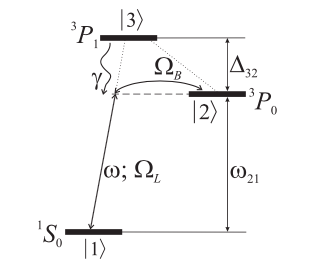
\includegraphics[scale=0.8]{figures/clock/energy_level}
	    \caption{(Adopted from ~\cite{Taichenachev06}) A small magnetic field breaks the LS coupling regime, and mixes \TPO ($\ket{3}$) \ and \TPZ($\ket{2}$) states, allowing otherwise forbidden transition from \SSZ to \TPZ.}
	    \label{fig:energy_level}
	\end{figure}
	%
	From~\cite{Taichenachev06}, the rabi frequency $\Omega$ for the \Sr{88} clock excitation is given by
	%
	\begin{align}
	\Omega&=\bra{\TPZ'}\mathbf{\hat{d}\cdot E}\ket{\SSZ}/\hbar=\frac{\Omega_L\Omega_B}{\Delta_{32}}\\
	&=\frac{\bra{\TPO}\mathbf{\hat{\mu}\cdot B}\ket{\TPZ}\bra{\TPO}\mathbf{\hat{d}\cdot E}\ket{\SSZ}}{\hbar^{2}\Delta_{32}}\\
	&=\frac{\langle\norm{\mu}\rangle\langle\norm{d}\rangle(\mathbf{E\cdot B)}} {\hbar^{2}\Delta_{32}}
	\end{align}
	%
	where $\langle\norm{\mu}\rangle$ and $\langle\norm{d}\rangle$ are reduced matrix elements. Using $\langle\norm{\mu}\rangle=\sqrt{2/3}\mu_{B}$ where $\mu_{B}$ is the Bohr magneton, $I=c\epsilon_{0}\abs{E}^{2}/2$, and $\langle\norm{d}\rangle$=0.151~\cite{cooper18}, the rabi frequency can be expressed in terms of the applied fields and light intensity
	%
	\begin{align}
		\Omega&=\alpha\sqrt{I}\abs{\textbf{B}}\text{cos}\theta
	\end{align}
	%
	\noindent where $\alpha$ is a measure of the induced Rabi frequency per unit of each of the fields, and $I$ is the light intensity, $\theta$ is the angle between linearly polarized $E$ and $B$ fields. Alternatively, $\Omega$ can be expressed in terms of the induced field shifts, the quadratic Zeeman $\Delta_B=\beta \textbf{B}^{2}$ and optical Stark $\Delta_L=\kappa I$ shifts where $\beta$ and $\kappa$ are respective shift coefficients, as 
	%
	\begin{align}
		\Omega=\xi\sqrt{\abs{\Delta_L \Delta_B}}\text{cos}\theta
	\end{align}
	%
	where $\xi\equiv\alpha/\sqrt{\beta\kappa}$. 

	


	% \begin{align}
	% 	\Omega&=\alpha\sqrt{I}\abs{\textbf{B}}\text{cos}\theta
	% \end{align}

	% \begin{center}
	% \begin{tabular}{ |c|c|c|c| } 
	% \hline
	% col1 & col2 & col3 \\
	% \hline
	% \multirow{3}{4em}{Multiple row} & cell2 & cell3 \\ 
	% & cell5 & cell6 \\ 
	% & cell8 & cell9 \\ 
	% \hline
	% \end{tabular}
	% \end{center}

